% Created 2016-05-21 Sat 20:16
\documentclass[9pt,b5paper]{article}
\usepackage{fontspec}
\setmainfont{STSong}
\usepackage{graphicx}
\usepackage{xcolor}
\usepackage{xeCJK}
\setCJKmainfont{STSong}
\usepackage{longtable}
\usepackage{float}
\usepackage{textcomp}
\usepackage{geometry}
\geometry{left=0cm,right=0cm,top=0cm,bottom=0cm}
\usepackage{multirow}
\usepackage{multicol}
\usepackage{listings}
\usepackage{algorithm}
\usepackage{algorithmic}
\usepackage{latexsym}
\usepackage{natbib}
\usepackage[xetex,colorlinks=true,CJKbookmarks=true,linkcolor=blue,urlcolor=blue,menucolor=blue]{hyperref}


\lstset{language=c++,numbers=left,numberstyle=\tiny,basicstyle=\ttfamily\small,tabsize=4,frame=none,escapeinside=``,extendedchars=false,keywordstyle=\color{blue!70},commentstyle=\color{red!55!green!55!blue!55!},rulesepcolor=\color{red!20!green!20!blue!20!}}
\author{deepwaterooo}
\date{\today}
\title{Tetris - Basic Implementation Practice for Android}
\hypersetup{
  pdfkeywords={},
  pdfsubject={},
  pdfcreator={Emacs 24.5.1 (Org mode 8.2.7c)}}
\begin{document}

\maketitle
\tableofcontents


\section{Upgrading versions, pretty good}
\label{sec-1}
\subsection{3d tetris}
\label{sec-1-1}
\subsubsection{Game Requirement}
\label{sec-1-1-1}
\begin{enumerate}
\item Model
\label{sec-1-1-1-1}
\begin{itemize}
\item So far draw, rotating has no issues. Just one more step to think after active block has rotated (90, 180, 270, 360 or whatever), after I droped, how am I going to put the correct element into board[i][j][k] matrix. I need rotation matrix calculation functions here for me to update my board. Data structure design I think it will work.
\begin{itemize}
\item Frame, Grid, and Cube needs to be design/packed better so that the rendering and rotations can be controlled slightly more organized.
\item Need to find a good/efficient way to manage and load all the sever different textures.
\end{itemize}
\item So far the only part that I want more research is on (Frame + Grid) vs current active block rotations, so that I could rotate them according when needed, (do I really need to use ray picking for identifying them) will do more online research on this part. I could implement ray picking, just feel 2d point doesn't necessarily fall into 3d frame. (which means outside 5*5*10 gestures to rotate frame, inside 5*5*10 frame rotate current active block, but I want more research to confirm if this is the best solution).
\end{itemize}
\item Threads
\label{sec-1-1-1-2}
\begin{itemize}
\item As you can feel once my mind is not clear I would make mistakes here or there. Threads/Runnables are useful but for opengl rendering because it is hardware accelerated rendering, unfortunately Threads/Runnables won't help too much for redering here. But I will try to pack these Threads/Runnables into my 2d tetris when this one is done. (think about it: if the thread calling opengl calls \textbf{setCurrentContext}. need to search more on opengl redering and thread for this module a little bit more. While concepts/ideas are right though. App developped in this age without threads applied I would feel shamed to call it a mobile app.) Need think about this part.
\item Threads for textures: 先解释下 glTexImage2d,它会将数据从 CPU 内存通过 PCIE 上传到 GPU 内存。不使用 PBO 时它是一个阻塞 CPU 的函数,数据量大时肯定会卡。解决方法是在子线程也创建一个 context,同时 share 资源给渲染的主线程。 
\begin{itemize}
\item \textbf{share$\backslash$$_{\text{context}}$:} Specifies another EGL rendering context with which to share data, as defined by the client API corresponding to the contexts. Data is also shared with all other contexts with which share$_{\text{context}}$ shares data. EGL$_{\text{NO}}$$_{\text{CONTEXT}}$ indicates that no sharing is to take place.

\lstset{language=c++,label= ,caption= ,numbers=none}
\begin{lstlisting}
EGLContext eglCreateContext(EGLDisplay display, EGLConfig config, EGLContext share_context, EGLint const * attrib_list);
\end{lstlisting}
\item 科普下 opengl 的线程不安全,它存了很多东西在线程的局部空间中,即 thread-local storage (TLS)。在没有绑定过 context (eglMakeCurrent / wglMakeCurrent)的线程中调用 opengl 函数是没有意义的,因为这个线程中嘛都没有。而一个 context 在同一时间只能被一个线程绑定。
\item 2种方法:(1) 2个线程, 1个OpenGL context,2个线程一个做渲染,一个做逻辑; (2), 2个线程2个context,主渲染线程维护状态,提交dc;辅助渲染线程做vb,texture的数据copy,shader的编译等。GPU会在两个context之间同步,有隐性开销. 其实单线程下规划好资源依赖应该可以做到不卡的.
\end{itemize}
\item 
\end{itemize}

\item Gestures
\label{sec-1-1-1-3}
\begin{itemize}
\item Includes MotionEvent for single finger, double or three fingers, use pointers, pack different gestures tasks into different runnables. gestures should be easy to use and apply. Look back on DrawingFun fun app developped during Fall 2014, fragments, threads, view/invalidates were all so easy, don't Understand why during those days I could only make them work without really/deeply understood how they works that way.
\begin{itemize}
\item In total about 15 gestions that I could think so far
\item 4 gestures for frame rotation around Z and x || (y = 2.5, z = 5) axis clockwise \&\& anti- for single finger touch (left, right, up, down).
\item 4 gestures for single finger active block moves up/dow x / y directions (left, right, up, down).
\item 6 gestures for double or triple fingers touch for acitve block rotates around x / y / z clock/anti-clockwise (left, right, up, down, 2 scrolls).
\item Double tap for fast dropping, but want to extend fast dropping gestures by applying velocities detection if I could figure those velocities out when the game flow is basically done.
\end{itemize}
\end{itemize}
\item Layout
\label{sec-1-1-1-4}
\begin{itemize}
\item The main activity game view allow NO buttons; If there are too many gestures applied, could include a instruction view for gesture guide. Could have slightly interesting layout for scores, or any effects that I could come up with later on (so far has not worried or do any research about this part yet).
\end{itemize}
\item Others
\label{sec-1-1-1-5}
\begin{itemize}
\item Minors features that I could skip if I don't have time:
\item After the bridgeing Cube app, texture is not any problems for me (just need to figure out a simple easier way to build an App manager (or simplier shaders) of my own, and manager the resources). Would borrow textures (with sounds) materials from glar3d and apply textures on my 3d game after majority functionalities are finished.
\item Come back to Cube app to make the mediaplayer for video work first, and then apply technic on Mediaplayer back to 3d for sounds besides the background sound, if I feel I have such a need with plants \&\& zombies Unity game waiting for me.
\item Expect the 3d game (videoable version) to be uploaded onto youtube by 5/17/2016. Considering debugging time and all other minor difficulties that I might meet later on, I will have to work hard on this one (Apparently I have not been able to finish by today then).
\end{itemize}
\end{enumerate}

\subsubsection{Status Update}
\label{sec-1-1-2}
\begin{itemize}
\item On the texture part for 3d, has NOT been able to compile yet, will continue work on it tomorrow.
\item 
\item On ray-picking, will try to temporarily apply it here to test and so that I could Understand this picking better, but I do think that I will need be scale(zoom out/in the frame so it will be more convenient to control current activeBlock) the frame to make it easy to use. But after I have learned all the technology I may not want to work on making it perfect any more. On textures loading. will continue with ray-picking in the evening.
\item need to set eye position better so that the (Frame + Grid) layout can be at the position that I want for the 3d game.
\item I want yellow grids, together with white background, red-x yellow-y, but I fail get such effect. Currently using black grid, but I will change it to be better looking.
\item Emacs is such a powerful tool for me for coding considering and accepting the facts that occasional it would produce some minor troubles for me so that I would have to google for solutions. This morning the parenthesis don't autopair for () [] \{\} for java-mode, after having googled for few minutes, I have used and trust autopair for so long and realized actually sometimes he gets tired, and once I close and restart it, he works perfectly. \textbf{I am looking forward to the day that my beloved cousin would be able to help and guide me with emacs debugging.}
\item 3d tetris layout structure:

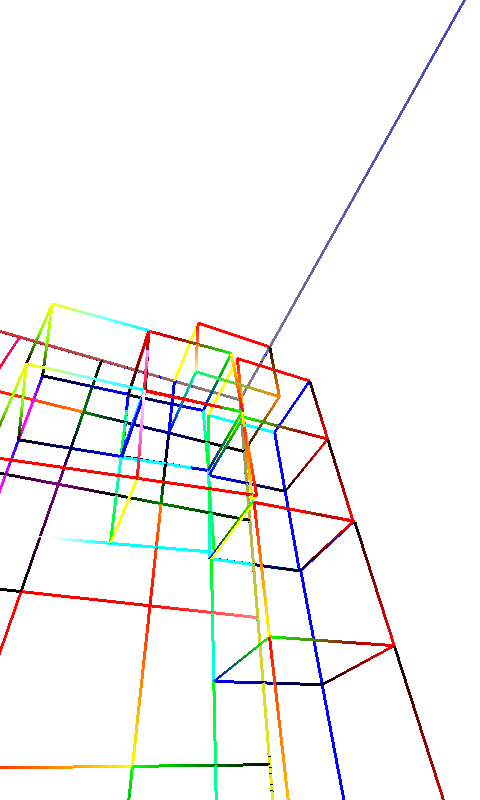
\includegraphics[width=.9\linewidth]{./pic/Screenshot_2016-05-12-12-06-42.png}
\item a video for this Tetris game can be directly watched at \url{https://www.youtube.com/watch?v=Ht4NOrEUtFk}
\item A video for the previous DrawingFun Android App can be watched at \url{https://www.youtube.com/watch?v=YV78Tk5--5M} , or by searching \textbf{deepwaterooo Wang}.
\end{itemize}

\subsection{folders}
\label{sec-1-2}
\begin{itemize}
\item lame2d: the very first version of the game.
\item 2d: SurfaceView redering 2d Implementation.
\item 3d: will work on a simple opengl 3d version first. Currently working on this one, will spend a few of following days on this one as well.
\item glar3d: upgraded opengl 3d version adapted from tetrisglar app with textures and music, and real 3d instead of any pseudo one, will implement this one when simple 3d version is done. (After having understood texture and lights better, tried to debug this one for a while, but still complicated design and layout still make this one to some extend difficult for me for now.)
\end{itemize}

\section{References}
\label{sec-2}
\subsection{youtube designs}
\label{sec-2-1}
\begin{itemize}
\item shader: \url{http://blog.csdn.net/tom_221x/article/details/38458021}
\item 旋转三角形 \url{http://www.hanshuliang.com/?post=6}
\item fancy effect: \url{http://m.oschina.net/blog/147033}
\item \url{http://www.cnblogs.com/liangliangh/p/4089582.html}
\item texture \url{http://learnopengl.com/code_viewer.php?code=getting-started/coordinate_systems&type=fragment}
\item github gestures explain details: \url{http://code.almeros.com/android-multitouch-gesture-detectors#.VzTg4BUrI9U}
\item shader abstract: \url{http://www.cnblogs.com/younghao/p/5141290.html}
\item shader thread \url{https://www.zhihu.com/question/28016196}
\item Activity \url{http://blog.csdn.net/luoshengyang/article/details/6685853} a series
\item Android线程管理 \url{http://www.cnblogs.com/younghao/p/5116819.html}
\item android share context \url{http://www.it610.com/article/3866383.htm}
\item three state rendering \url{https://www.youtube.com/watch?v=t5EeXKGSQUw}
\item \url{http://blog.slapware.eu/game-engine/programming/multithreaded-renderloop-part1/}
\item \url{https://www.hongweipeng.com/index.php/archives/581/}
\item \url{https://github.com/lp0/slf4j-android/tree/master/src/main/java/eu/lp0/slf4j/android}
\item \url{http://www.cnblogs.com/younghao/p/5141290.html}
\item \url{http://mobile.51cto.com/aengine-437172.htm}
\item \url{http://www.jianshu.com/p/291ff6ddc164}
\item shaders: \url{https://github.com/learnopengles/Learn-OpenGLES-Tutorials/blob/master/android/AndroidOpenGLESLessons/src/com/learnopengles/android/common/ShaderHelper.java}
\item 
\item 
\item 
\item 
\item 
\item 
\item 
\end{itemize}

\subsection{gestures}
\label{sec-2-2}
\begin{itemize}
\item 过程\url{https://wizardforcel.gitbooks.io/w3school-android/content/62.html}
\item analyze with code \url{https://github.com/CharonChui/AndroidNote/blob/master/Android\%E5\%8A\%A0\%E5\%BC\%BA/Android\%20Touch\%E4\%BA\%8B\%E4\%BB\%B6\%E5\%88\%86\%E5\%8F\%91\%E8\%AF\%A6\%E8\%A7\%A3.md}
\item android MotionEvent 详解 pointers \url{http://www.jianshu.com/p/0c863bbde8eb}
\item 图片过程详解\url{http://ztelur.github.io/2016/02/04/\%E5\%9B\%BE\%E8\%A7\%A3Android\%E4\%BA\%8B\%E4\%BB\%B6\%E4\%BC\%A0\%E9\%80\%92\%E4\%B9\%8BView\%E7\%AF\%87/} check github scrollview
\item \url{http://www.jianshu.com/p/293d0c2f56cb} Android 绘制过程详解
\item Track Velocity \url{http://developer.android.com/intl/zh-cn/training/gestures/movement.html#velocity}
\item sample codes: \url{https://gitlab.com/tgzzl/android-training-course-in-chinese/blob/0727674297209b5d89db01ee768da1db1ac6cea0/input/gestures/detector.md}
\item Drag and Drop \url{http://developer.android.com/intl/zh-cn/guide/topics/ui/drag-drop.html}
\item 拖拽与缩放 \url{http://hukai.me/android-training-course-in-chinese/input/gestures/scale.html} 更加复杂的缩放示例
\item 滚动手势动画 \url{http://hukai.me/android-training-course-in-chinese/input/gestures/scroll.html}
\item 响应触摸事件 \url{http://hukai.me/android-training-course-in-chinese/graphics/opengl/touch.html}
\item 多线程操作 \url{http://hukai.me/android-training-course-in-chinese/performance/multi-threads/index.html}
\item Android入门基础 \url{http://hukai.me/android-training-course-in-chinese/basics/index.html}
\item example code Android 中实现图片平移、缩放、旋转同步进行 \url{http://android.jobbole.com/82072/}
\item another ray picking: \url{http://antongerdelan.net/opengl/raycasting.html}
\item opengl es rendering vs threads: \url{http://imgtec.eetrend.com/blog/1883}
\item bash globstar ** \url{http://smilejay.com/2013/10/enable-globstar-in-bash/}
\item 调试 \url{http://gold.xitu.io/entry/56c5d052a34131005005f55e}
\item youtube gestures 定义:\url{https://www.youtube.com/watch?v=ZJj-9HqRpDc}
\item GLSurfaceView \url{http://hellosure.github.io/android/2015/06/01/android-glsurfaceview/}
\item handling touch thread \& rendering threads \url{http://stackoverflow.com/questions/5129580/android-glsurfaceview-renderer-is-interrupting-an-incomplete-touch-event}
\item \url{http://www.learnopengles.com/listening-to-android-touch-events-and-acting-on-them/}
\item github 3d tetris reference \url{https://github.com/kdomic/android-3d-tetris}
\end{itemize}

\subsection{Activity.runOnUiThread()}
\label{sec-2-3}
\begin{itemize}
\item \url{http://stackvoid.com/introduction-to-Message-Handler-in-Android/}
\item \url{http://m.oschina.net/blog/97619}
\item AssetManager: \url{http://m.jb51.net/article/57341.htm}
\item A 3d reference: \url{https://github.com/kdomic/android-3d-tetris}
\end{itemize}
\subsection{3D design}
\label{sec-2-4}
\begin{itemize}
\item c++ version: \url{https://github.com/matachi/tetris-cpp}
\item refer 6 \url{http://www.oschina.net/question/614942_62370}
\item \url{http://www.oschina.net/question/565065_67280}
\item triangle: \url{http://stackoverflow.com/questions/9945321/triangle-opengl-in-android}
\item \url{https://gist.github.com/SebastianJay/3316001}
\item 射线拾取: \url{http://itdocument.com/479827008/}
\item 旋转及手势: \url{http://vaero.blog.51cto.com/4350852/790620}
\item 2 \url{http://vaero.blog.51cto.com/4350852/790637}
\item \url{http://www.lai18.com/content/951343.html}
\item opengl选择与反馈: \url{http://zhidao.baidu.com/question/496046750245095004.html}
\item \url{http://wenku.baidu.com/view/58190d1efad6195f312ba6f7.html}
\item c++ \url{http://blog.csdn.net/u010223072/article/details/45369075}
\item \url{http://codercdy.com/2015/06/17/openglxue-xi-bi-ji-xuan-ze-he-fan-kui/}
\item \url{https://books.google.com/books?id=u6EHM_OzaFQC&pg=PA1987&lpg=PA1987&dq=opengl\%E9\%80\%89\%E6\%8B\%A9\%E4\%B8\%8E\%E5\%8F\%8D\%E9\%A6\%88&source=bl&ots=L9Y66QSEhu&sig=f1h_RadXRDFsa9L5IY430HGTG34&hl=en&sa=X&ved=0ahUKEwjA6vTRo_jLAhVH3mMKHQIXBxYQ6AEIPDAE#v=onepage&q=opengl\%E9\%80\%89\%E6\%8B\%A9\%E4\%B8\%8E\%E5\%8F\%8D\%E9\%A6\%88&f=false}
\item c++ codes: \url{http://dev.gameres.com/program/Visual/3D/Selection.htm}
\item 画线: c++ \url{http://www.programgo.com/article/43724048060/}
\item draw line: \url{http://www.linuxidc.com/Linux/2011-09/42307p3.htm}
\item \url{http://stackoverflow.com/questions/9217702/open-gl-es-2-0-drawing-a-simple-line}
\item 距阵变换: \url{http://www.cnblogs.com/caster99/p/4780984.html}
\item \url{http://www.flakor.cn/2014-05-15-384.html}
\item shader util: \url{http://blog.csdn.net/shulianghan/article/details/17020359}
\item 详解距阵变换:\url{http://www.cnblogs.com/kesalin/archive/2012/12/06/3D_math.html}
\item \url{http://mail.cfanz.cn/index.php?c=article&a=read&id=270244}
\item one example: \url{http://www.apkbus.com/blog-99192-39498.html}
\item ex2 for shader matrix: \url{http://www.voidcn.com/blog/peanut__love/article/p-2891341.html}
\item 西蒙iPhone-OpenGL ES 中文教程专题: \url{http://www.cocoachina.com/special/2010/0126/404.html}
\item 运动: \url{http://www.cocoachina.com/bbs/read.php?tid-7601-fpage-10.html}
\item 距阵: \url{http://blog.csdn.net/wangdingqiaoit/article/details/39010077}
\item \url{http://blog.csdn.net/popy007/article/details/5120158} UNV
\item \url{http://www.tqcto.com/article/mobile/23873.html} eye
\item \url{http://blog.csdn.net/wangdingqiaoit/article/details/39937019}
\item \url{https://developer.apple.com/library/ios/documentation/3DDrawing/Conceptual/OpenGLES_ProgrammingGuide/Introduction/Introduction.html}
\item \url{http://blog.csdn.net/shulianghan/article/details/46680803}
\item rotation: \url{http://stackoverflow.com/questions/13480043/opengl-es-android-matrix-transformations}
\item glsl example: \url{http://cse.csusb.edu/tongyu/courses/cs520/notes/android-es2.php}
\item shader parser: \url{http://stackoverflow.com/questions/19452240/opengl-glsl-void-parse-error-on-vertex-shader}
\item separate file: \url{http://stackoverflow.com/questions/30345816/splitting-a-text-file-into-multiple-files-by-specific-character-sequence}
\end{itemize}
\subsection{GLSurfaceView}
\label{sec-2-5}
\begin{itemize}
\item opengl: \url{http://androidblog.reindustries.com/a-real-open-gl-es-2-0-2d-tutorial-part-1/}
\item Graphics architecture: \url{https://source.android.com/devices/graphics/architecture.html}
\item \url{http://stackoverflow.com/questions/5169338/android-deciding-between-surfaceview-and-opengl-glsurfaceview}
\item \textbf{引路蜂} better: \url{http://blog.csdn.net/mapdigit/article/details/7526556}
\item 真正的3D图形: \url{http://www.imobilebbs.com/wordpress/archives/1554}
\item a Cube: \url{http://www.oschina.net/question/4873_28325}
\item modification: \url{https://github.com/googleglass/gdk-apidemo-sample/blob/master/app/src/main/java/com/google/android/glass/sample/apidemo/opengl/Cube.java}
\item Android OpenGL ES 简明开发教程小结: \url{http://www.imobilebbs.com/wordpress/archives/1583}
\item \url{http://hellosure.github.io/android/2015/06/01/android-glsurfaceview/}
\item \url{http://ju.outofmemory.cn/entry/172850}
\item 画图: \url{http://www.mobile-open.com/2015/81568.html}
\item \url{http://tangzm.com/blog/?p=20}
\item \url{http://www.apkbus.com/blog-99192-39584.html}
\item onDrawFrame intro: \url{http://www.jayway.com/2009/12/03/opengl-es-tutorial-for-android-part-i/}
\item failed: \url{http://stackoverflow.com/questions/28711850/android-opengl-how-to-draw-a-rectangle}
\item onTouchEvent: \url{http://blog.csdn.net/niu_gao/article/details/8673662}
\item volatile \url{http://www.voidcn.com/blog/fanfanxiaozu/article/p-3668133.html}
\item \url{http://mobile.51cto.com/aengine-437172.htm}
\item OpenGLES related: \url{http://stackoverflow.com/questions/9945321/triangle-opengl-in-android}
\item OpenGL ES 2.0 Sample Code: \url{http://androidbook.com/item/4254}
\item intros:详解 \url{http://blog.csdn.net/niu_gao/article/details/7566297}
\item 画线: \url{http://www.cnblogs.com/lhxin/archive/2012/06/01/2530828.html}
\item \url{http://bbs.9ria.com/thread-201740-1-1.html}
\item \url{http://imgtec.eetrend.com/blog/5078}
\item draw a ball \url{http://shikezhi.com/html/2015/android_1022/561912.html}
\item for Board c++: \url{http://www.jiancool.com/article/24471349949/}
\item possible? \url{http://code1.okbase.net/codefile/CCFormatter.java_2015072733469_393.htm}
\item \url{http://www.mobile-open.com/2015/80379.html}
\end{itemize}
\subsection{eventQueue vs SurfaceView threads}
\label{sec-2-6}
\begin{itemize}
\item Deeper summary, android graphics architecture: \url{http://hukai.me/android-deeper-graphics-architecture/}
\item 2 threads, load, read, \url{http://blog.csdn.net/hellogv/article/details/5986835}
\end{itemize}
\subsection{SurfaceView}
\label{sec-2-7}
\begin{itemize}
\item Surface runnable \url{http://android.okhelp.cz/surfaceview-implements-runnable-android-code/}
\item Example: \url{http://technicalsearch.iteye.com/blog/1967616}
\item \url{http://www.jcodecraeer.com/a/anzhuokaifa/androidkaifa/2012/1201/656.html}
\item Event Queue: \url{http://www.leestorm.com/post/17.html}
\item lockCanvas(Rect小区) \url{http://blog.csdn.net/alexander_xfl/article/details/13000347}
\item example: \url{http://fanli7.net/a/JAVAbiancheng/ANT/20120424/160203.html}
\item MotionEvent: \url{http://android.jobbole.com/82072/}
\item surfaceview双缓冲: \url{http://blog.csdn.net/cnbloger/article/details/7404485}
\item sth worth try: \url{http://www.lxway.com/969295592.htm}
\item Dont Understand: \url{http://blog.sina.com.cn/s/blog_5a6f39cf01012rtv.html}
\item tried: \url{http://bbs.csdn.net/topics/370074255} drawBitmap 2 canvas
\item slightly complicated: \url{http://www.lxway.com/148606691.htm}
\item slightly complicated: \url{http://www.lxway.com/186948856.htm}
\end{itemize}
\subsection{gestures}
\label{sec-2-8}
\begin{itemize}
\item \url{http://www.cnblogs.com/akira90/archive/2013/03/10/2952886.html}
\item Android 触摸手势基础 官方文档概览: \url{http://www.lxway.com/445554926.htm}
\item 手势: \url{http://wiki.jikexueyuan.com/project/material-design/patterns/gestures.html}
\item \url{http://www.lxway.com/601620614.htm}
\item \url{http://www.lxway.com/282219004.htm}
\item \url{http://www.lxway.com/906451412.htm}
\item \url{http://www.lxway.com/146619692.htm}
\item \url{http://www.lxway.com/4420294641.htm}
\item \url{http://www.lxway.com/155059816.htm}
\item \url{http://www.lxway.com/4019928952.htm}
\item 例子: \url{http://bbs.chinaunix.net/thread-3634477-1-1.html}
\item 例子: \url{http://www.bestappsmarket.com/p/app?appId=1192877&title=tetris-\%E4\%BF\%84\%E7\%BD\%97\%E6\%96\%AF\%E6\%96\%B9\%E5\%9D\%97}
\item 例子: \url{http://bbs.chinaunix.net/thread-3634477-1-1.html}
\item iTetris: \url{http://searchapp.soft4fun.net/article/information/iTetris\%20\%E4\%BF\%84\%E7\%BD\%97\%E6\%96\%AF\%E6\%96\%B9\%E5\%9D\%97/313319}
\item left right: \url{http://www.jb51.net/article/77028.htm}
\item AI: \url{http://www.cnblogs.com/youngshall/archive/2009/03/24/1420682.html}
\item 3/11/2016 Friday
\item \url{https://github.com/Almeros/android-gesture-detectors} mac
\item \url{http://www.jcodecraeer.com/a/anzhuokaifa/androidkaifa/2015/0211/2467.html}
\item \url{http://www.hejun.biz/81.html}
\item \url{http://www.jb51.net/article/38166.htm}
\item \url{http://www.jb51.net/article/37717.htm}
\item \url{http://mobile.51cto.com/aprogram-394841.htm}
\item TetrisBattle特殊轉入教學(Z S J L I)
\begin{itemize}
\item \url{https://www.youtube.com/watch?v=zW6Gp_7jl9I}
\end{itemize}
\item 推箱子: 第11章 Android游戏开发视频教程 益智游戏——推箱子
\begin{itemize}
\item \url{https://www.youtube.com/watch?v=glzxII1-P0A} 2.5D
\end{itemize}
\item 祖码游戏的设计与实现
\end{itemize}
% Emacs 24.5.1 (Org mode 8.2.7c)
\end{document}